\section{Discrete-scan dispersion and the ``speed of light'' question}
\label{sec:dispersion}

This section isolates one concrete, model-level interface between the scan formalism and phenomenology: the exact dispersion relation induced by a discrete scan/difference replacement.
The goal is not to claim a unique physical prediction, but to provide a falsifiable template: any scan-based lattice model carries characteristic high-energy deviations from linear propagation.

\subsection{A representative exact dispersion relation}
In the HPA scan calculus, replacing derivatives by finite differences at step size $\varepsilon$ yields an exact lattice-type dispersion of the form \cite{Ma2025HPA}
\begin{equation}
E(P)=\frac{2}{\varepsilon}\arcsin\!\left(\frac{\varepsilon P}{2}\right).
\label{eq:lattice_dispersion}
\end{equation}
For $\varepsilon P\ll 1$, the low-energy expansion is
\begin{equation}
E(P)=P+\frac{\varepsilon^2 P^3}{24}+O(\varepsilon^4 P^5),
\label{eq:lattice_dispersion_low_energy}
\end{equation}
so linear propagation is recovered to leading order.

\subsection{Derivation via the symbol of a symmetric difference}
A compact derivation uses the standard Fourier symbol of the symmetric difference.
Let the symmetric difference operator be
\begin{equation}
(\nabla_{\varepsilon} f)(t):=\frac{f(t+\varepsilon/2)-f(t-\varepsilon/2)}{\varepsilon}.
\end{equation}
For a plane wave $f(t)=\exp(-\iu E t)$ one has
\begin{equation}
\nabla_{\varepsilon}\,\exp(-\iu E t)=-\iu\,\widetilde{E}(E)\,\exp(-\iu E t),
\qquad \widetilde{E}(E):=\frac{2}{\varepsilon}\sin\!\left(\frac{\varepsilon E}{2}\right).
\end{equation}
Imposing the continuum massless dispersion $E=P$ at the level of symbols by setting $\widetilde{E}(E)=P$ gives
\begin{equation}
\sin\!\left(\frac{\varepsilon E}{2}\right)=\frac{\varepsilon P}{2},
\end{equation}
which solves to Equation~\eqref{eq:lattice_dispersion}.

\subsection{MDR form and the quadratic suppression scale}
Squaring the low-energy expansion gives a convenient modified-dispersion-relation (MDR) form:
\begin{equation}
E^2 = P^2 + \frac{\varepsilon^2}{12}P^4 + O(\varepsilon^4 P^6).
\label{eq:mdr_quadratic}
\end{equation}
Define the quadratic suppression scale
\begin{equation}
E_{\mathrm{QG},2}:=\frac{\sqrt{12}}{\varepsilon}.
\label{eq:eqg2_def}
\end{equation}
Then
\begin{equation}
E^2 = P^2\left[1+\left(\frac{P}{E_{\mathrm{QG},2}}\right)^2+O\!\left(\frac{P^4}{E_{\mathrm{QG},2}^4}\right)\right].
\end{equation}
This places the scan-induced dispersion directly into the standard quadratic LIV/MDR phenomenology vocabulary.

\subsection{Group velocity and high-energy deviation}
Differentiating \eqref{eq:lattice_dispersion} gives
\begin{equation}
\frac{dE}{dP}=\frac{1}{\sqrt{1-(\varepsilon P/2)^2}}.
\label{eq:group_velocity}
\end{equation}
Thus, the scan-induced dispersion predicts an energy-dependent deviation from constant group velocity.
In particular, for $\varepsilon P\ll 1$,
\begin{equation}
\frac{dE}{dP}=1+\frac{\varepsilon^2 P^2}{8}+O(\varepsilon^4 P^4)
\ =\ 1+\frac{3}{2}\left(\frac{P}{E_{\mathrm{QG},2}}\right)^2+\cdots.
\end{equation}

\begin{figure}[t]
\centering
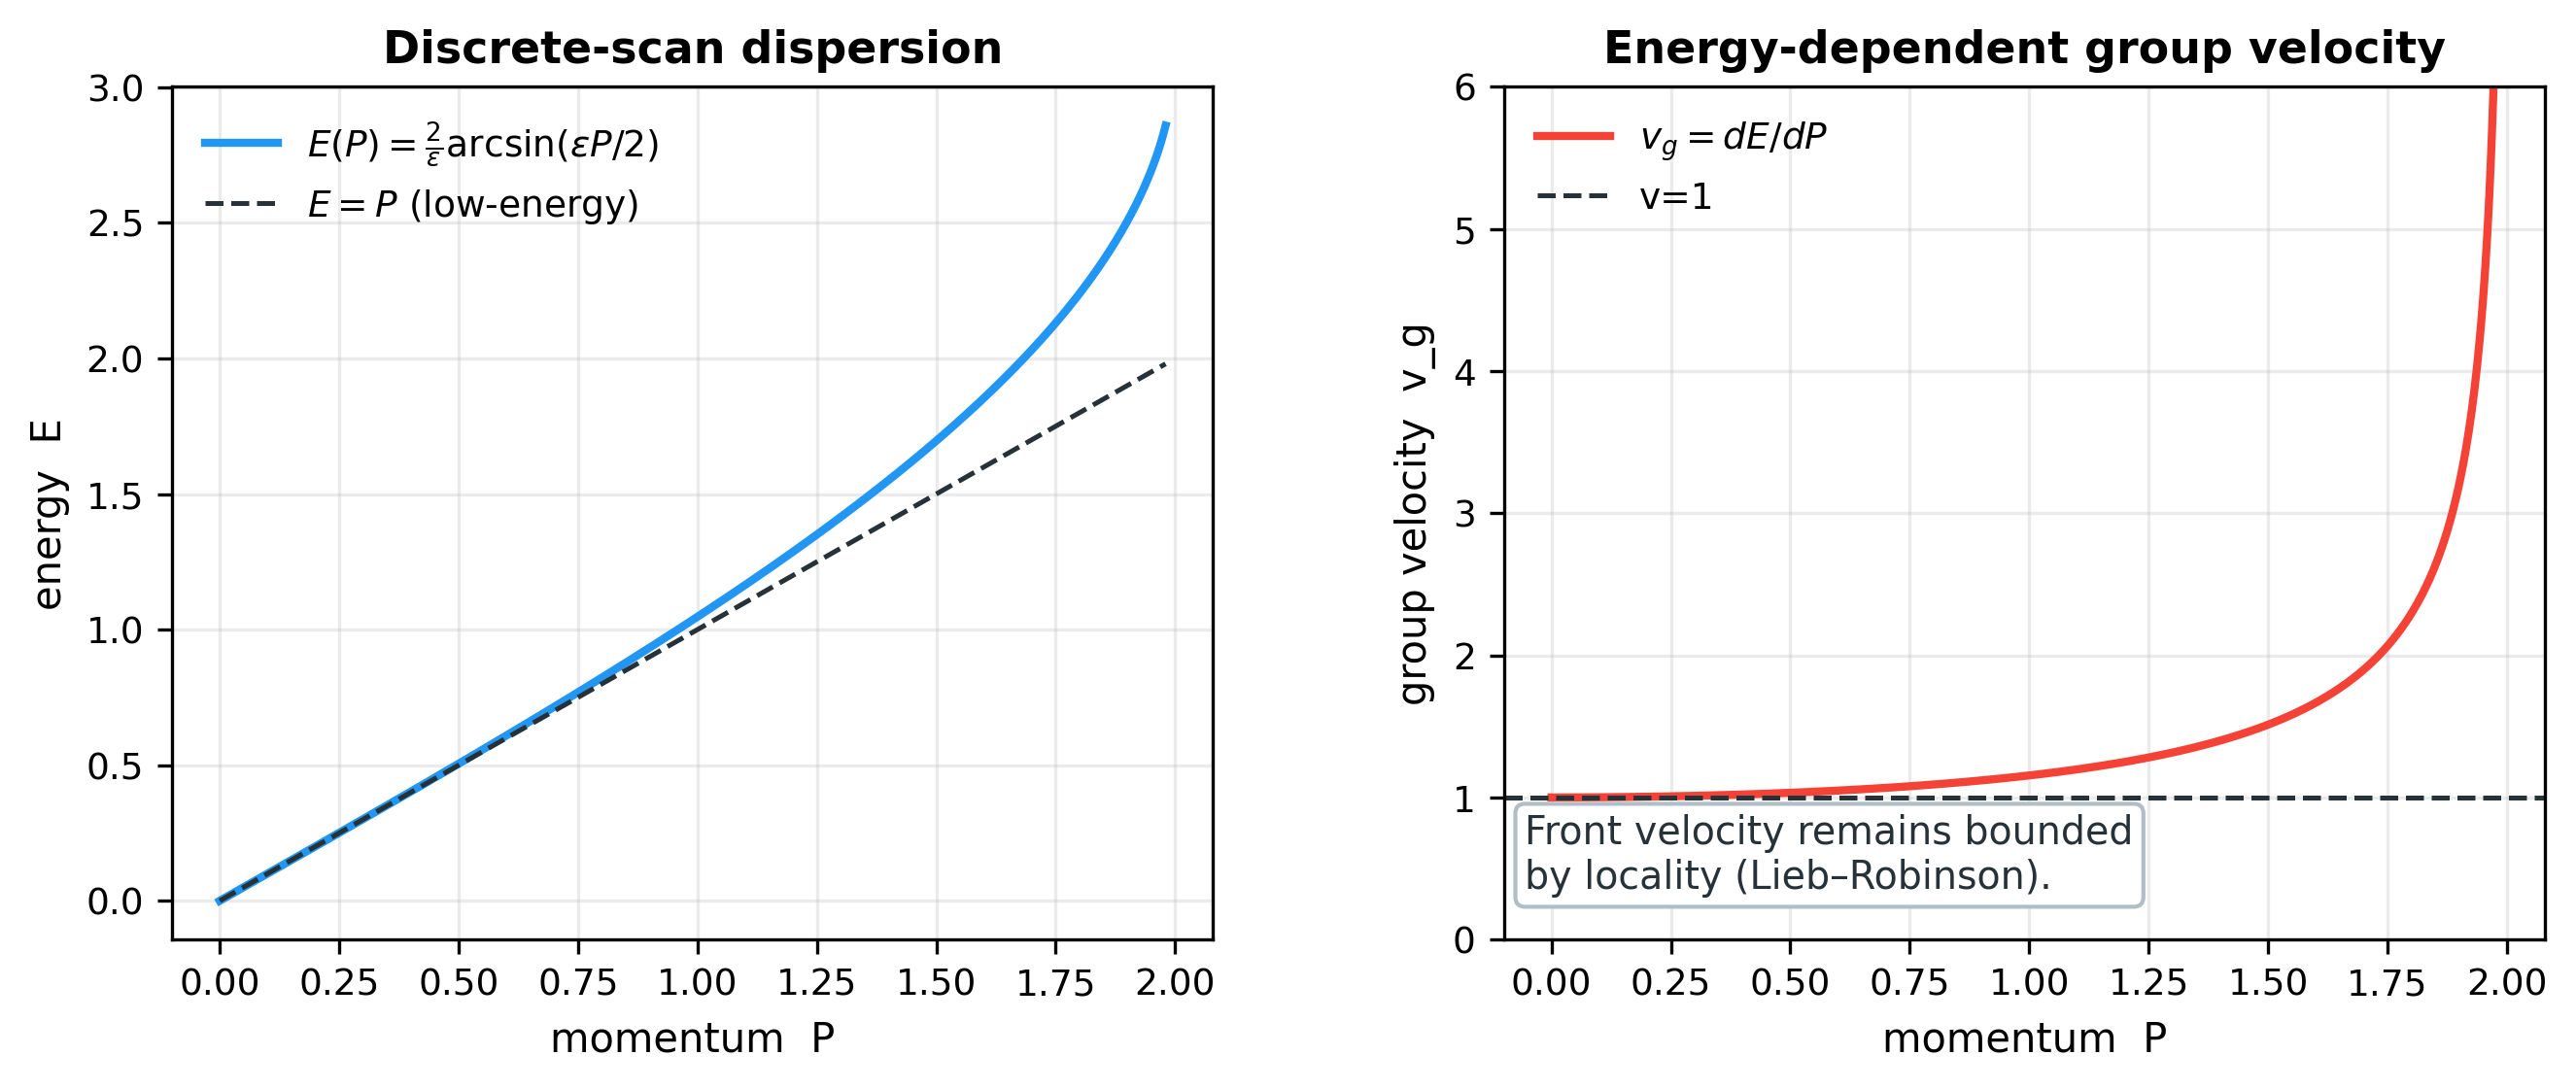
\includegraphics[width=0.98\textwidth]{images/fig5_dispersion.png}
\caption{\textbf{Discrete-scan dispersion and energy-dependent group velocity.} The exact scan-induced dispersion $E(P)=\frac{2}{\varepsilon}\arcsin(\varepsilon P/2)$ is approximately linear at low energy and deviates at high momentum. The corresponding group velocity $v_g=dE/dP$ becomes energy-dependent; microscopic locality in a QCA/PQCA imposes a separate signal/front-velocity bound (Lieb--Robinson).}
\label{fig:dispersion}
\end{figure}

\subsection{Cosmological time-of-flight fitting (quadratic case)}
For a source at redshift $z$ in a standard FRW background, the leading quadratic time-delay template takes the familiar form \cite{JacobPiran2008}:
\begin{equation}
\Delta t_{\mathrm{LIV}}\ \simeq\ s_2\,\frac{3}{2}\,\frac{E_{\mathrm{h},0}^2-E_{\mathrm{l},0}^2}{E_{\mathrm{QG},2}^2}\int_0^z\frac{(1+z')^2}{H(z')}\,dz',
\label{eq:tof_quadratic}
\end{equation}
where $E_{\mathrm{h},0},E_{\mathrm{l},0}$ are the observed photon energies and $s_2\in\{+1,-1\}$ encodes subluminal vs superluminal sign conventions.
Here $H(z)$ is the Hubble parameter; for a spatially flat $\Lambda$CDM background one may take
\begin{equation}
H(z)=H_0\sqrt{\Omega_m(1+z)^3+\Omega_\Lambda}.
\end{equation}
In the scan dispersion \eqref{eq:lattice_dispersion}, the quadratic correction is superluminal (positive $dE/dP-1$), corresponding to a fixed sign choice in this template.

Equation~\eqref{eq:tof_quadratic} provides a direct fitting pipeline: given $(\Delta t_i,E_{\mathrm{h},0,i},E_{\mathrm{l},0,i},z_i)$ one can regress for $E_{\mathrm{QG},2}$ (equivalently $\varepsilon$ via \eqref{eq:eqg2_def}) subject to astrophysical emission-lag systematics.

\subsection{A concrete bound (example)}
Using Fermi-LAT gamma-ray burst data, Vasileiou \emph{et al.}\ reported a robust quadratic constraint of order
\begin{equation}
E_{\mathrm{QG},2} > 1.3\times 10^{11}\,\mathrm{GeV}
\end{equation}
within their systematic treatment \cite{Vasileiou2013} (see also the earlier GRB~090510 limit \cite{Abdo2009Nature}).
Translating via \eqref{eq:eqg2_def} gives the corresponding bound on the scan step
\begin{equation}
\varepsilon < \frac{\sqrt{12}}{1.3\times 10^{11}\,\mathrm{GeV}}\approx 2.7\times 10^{-11}\,\mathrm{GeV}^{-1}.
\end{equation}
In length units, $1\,\mathrm{GeV}^{-1}\simeq 1.97\times 10^{-16}\,\mathrm{m}$, so $\varepsilon\lesssim 5.3\times 10^{-27}\,\mathrm{m}$.

\subsection{Causality: group velocity vs signal velocity}
Equation~\eqref{eq:group_velocity} can exceed $1$ for sufficiently large $P$.
However, in a strictly local update model (QCA/PQCA), information propagation is bounded by locality: per tick, influence can spread only within a finite neighborhood.
In fact, for a causal QCA with neighborhood radius $r$, the Heisenberg evolution obeys a \emph{strict} light-cone statement \cite{ArrighiNesmeWerner2011}:
\begin{equation}
\mathrm{supp}\!\left(U^{\dagger}A_XU\right)\subseteq \mathcal{N}_r(X),
\end{equation}
for any observable $A_X$ supported on a finite set $X$, where $\mathcal{N}_r(X)$ denotes the $r$-neighborhood of $X$ in graph distance.
Iterating gives $\mathrm{supp}(U^{-t}A_XU^t)\subseteq \mathcal{N}_{rt}(X)$, so the front/signal velocity is bounded by the microscopic causality radius.
For more general local quantum dynamics generated by Hamiltonians, strict causality is replaced by an exponentially suppressed tail outside an effective cone, formalized by Lieb--Robinson bounds \cite{LiebRobinson1972}.
Therefore, an apparent ``superluminal group velocity'' extracted from a lattice dispersion must be interpreted cautiously: group velocity is not a signal-velocity guarantee, while the microscopic locality constraint enforces the true causal speed limit.

\subsection{How this connects back to complexity}
In the unified semantics, the effective propagation speed is determined by the scan step and by the compilation overhead required to realize local updates.
Hence, ``light-cone structure'' is itself a complexity statement: it is a bound on how many sites can be causally reached within a given depth budget.
This ties the phenomenological dispersion discussion back to the central theme: kinematics is constrained by scan complexity (iteration/depth) and by readout resolution (which determines which deviations are operationally accessible).
